

In this \headerName{}, we present the results of our training experiments, and provide insights on them.


%Due to space constraints, we're unable to display all the metrics from the training data. 
Comprehensive training plots and logs can be found in our GitLab repository. For a glimpse into the results from our initial training round, refer to Figures \ref{fig:07_vsi_sample_training_logs_unbalanced} and \ref{fig:07_vsi_sample_training_logs_pet_1000}. 
In the first figure, we can see that the optimal epoch to avoid overfitting in that particular scenario is the fourth epoch, which coincidentally also maximizes the \fTwo{}. 
In contrast, in the second image, the first epoch is optimal, while it does not have the best \fTwo{}.



\begin{figure}[ht]
    \centering
    \subfigure[Training Loss]{
            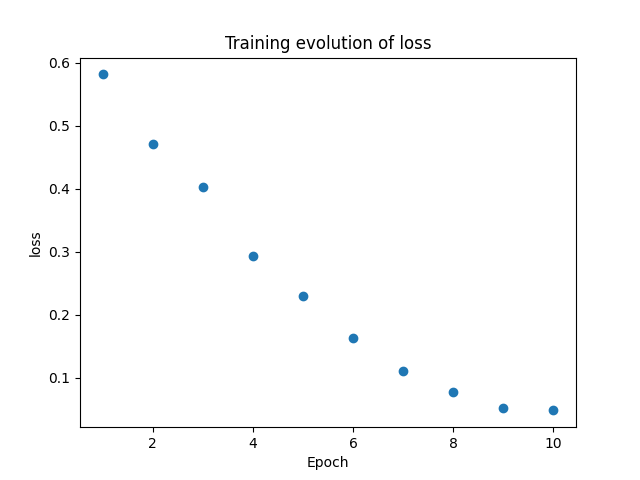
\includegraphics[width=0.3\textwidth]{Figures/07/sample_result/unbalanced_mbert_trafilatura_title_loss.png}
    }
    \hfill
    \subfigure[Development Loss]{
            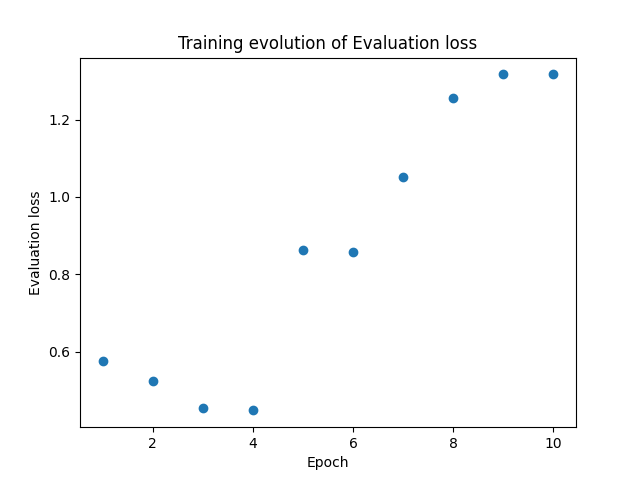
\includegraphics[width=0.3\textwidth]{Figures/07/sample_result/unbalanced_mbert_trafilatura_title_eval_loss.png}
    }
    \hfill
    \subfigure[Development \fTwo{}]{
            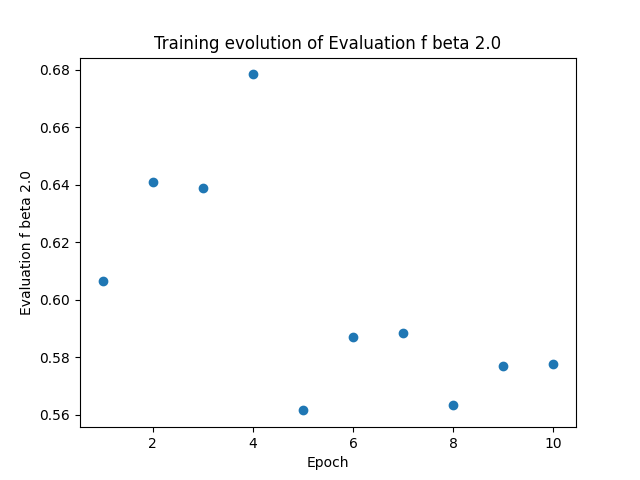
\includegraphics[width=0.3\textwidth]{Figures/07/sample_result/unbalanced_mbert_trafilatura_title_eval_f_beta_2.0.png}
    }
    \caption{\unbalanced{} - Losses and Development \fTwo{} evolution for \bertmultilingual{} on the \trafilaturaTitle{}}
    \label{fig:07_vsi_sample_training_logs_unbalanced}
\end{figure}


\begin{figure}[ht]
    \centering
    \subfigure[Training Loss]{
            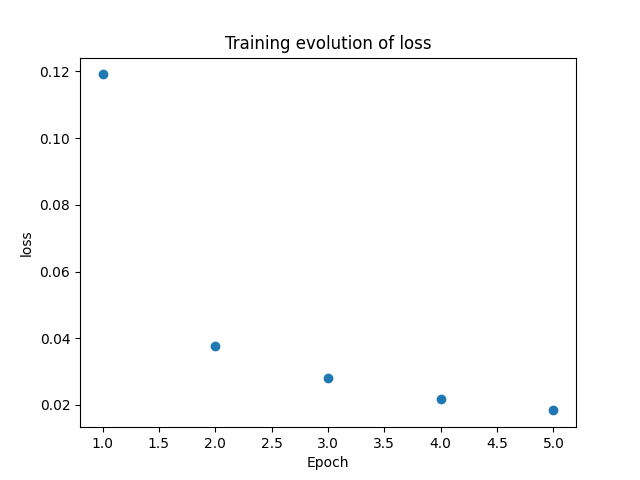
\includegraphics[width=0.3\textwidth]{Figures/07/sample_result/pet1000_roberta_trafilatura_title_loss.png}
    }
    \hfill
    \subfigure[Development Loss]{
            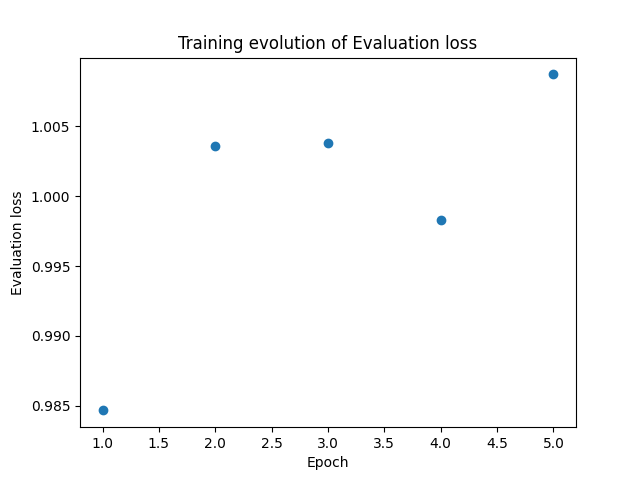
\includegraphics[width=0.3\textwidth]{Figures/07/sample_result/pet1000_roberta_trafilatura_title_eval_loss.png}
    }
    \hfill
    \subfigure[Development \fTwo{}]{
            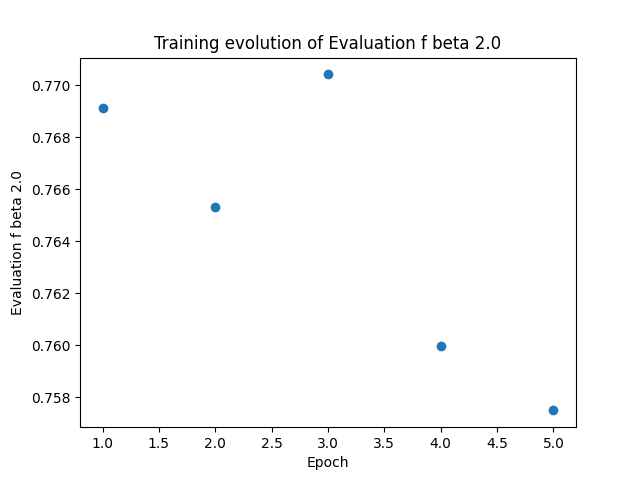
\includegraphics[width=0.3\textwidth]{Figures/07/sample_result/pet1000_roberta_trafilatura_title_eval_f_beta_2.0.png}
    }
    \caption{\petThousand{} - Losses and Development \fTwo{} evolution for \bertroberta{} on the \trafilaturaTitle{}}
    \label{fig:07_vsi_sample_training_logs_pet_1000}
\end{figure}



The optimal epochs for each training scenario are detailed in \appendixname{} \ref{appendix05:vsi_optimal_epochs}. It's evident that \unbalanced{} takes the longest to reach the optimal epoch, especially when compared to the other methods, where the majority reach the optimum within the first or second epoch. The disparity between the two fine-tuning techniques is significant, with \balanced{} often reaching its peak performance in just one epoch. When it comes to \gls{pet}, all five scenarios exhibit a consistent pattern, typically achieving their optimal epoch before the fourth one. This suggests that any variations in the rate of convergence might occur during the training of the \gls{pet} ensembles. Given that all ensembles undergo training for five epochs, it must be that this sufficient for achieving satisfactory results. Unfortunately, we did not record the evolution of the custom losses used to train the \gls{pet} ensembles.


\begin{figure}[ht]
    \centering
    \subfigure{
            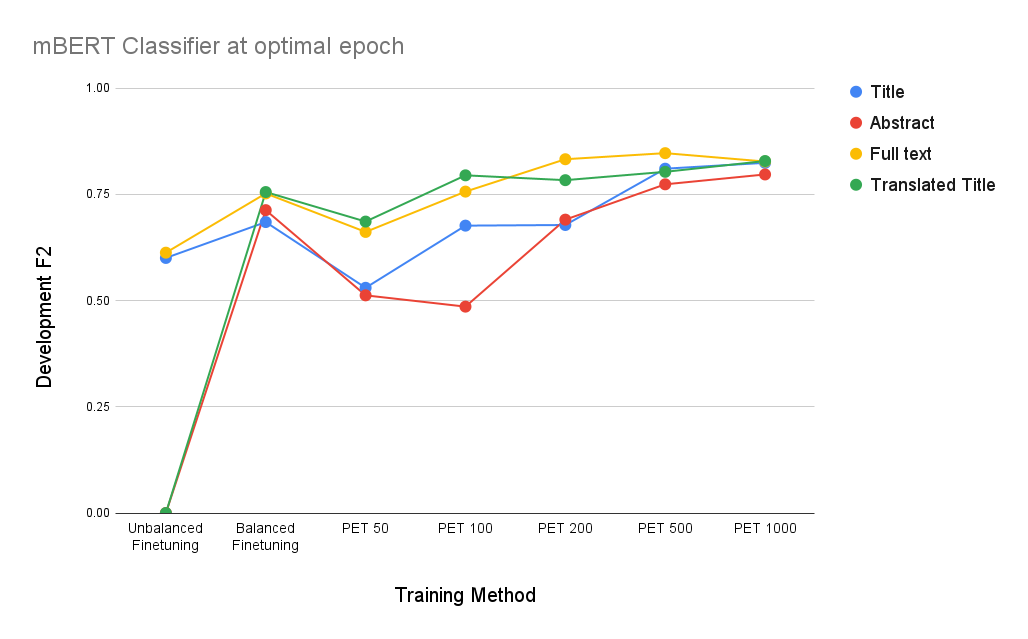
\includegraphics[width=0.45\textwidth]{Figures/07/mBERT Classifier at optimal epoch_trafilatura.png}
    }
    %\hfill
    \subfigure{
            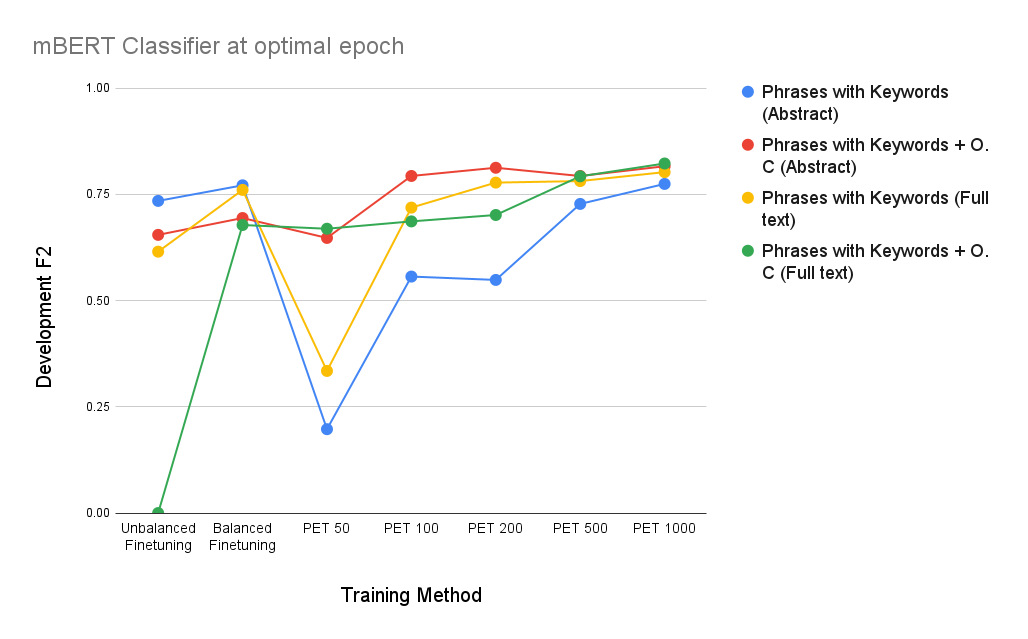
\includegraphics[width=0.45\textwidth]{Figures/07/mBERT Classifier at optimal epoch_keyphrases.png}
    }
    \caption{Development \fTwo{} for \bertmultilingual{} at the optimal epochs, across all the training methods}
    \label{fig:07_dev_f2_mbert}
\end{figure}

Based on these findings, we moved forward to the second round, trained models up to their optimal epochs, and evaluated their final performance.
The metrics for the best classifiers across each training scenario and for every \gls{bert} model are detailed in \appendixname{} \ref{appendix05:vsi_metrics_optimal_epochs}. 
A direct comparison of the Development \fTwo{} outcomes reveals that \unbalanced{} consistently underperforms compared to other training techniques
\footnote{A \fTwo{} score of 0\% indicates the model defaulted to predict the predominant class (negative)} (See Figure \ref{fig:07_dev_f2_mbert} for sample results for \bertmultilingual{}).
In fact, \balanced{} outperforms \unbalanced{} in nearly all instances, with only one exception\footnote{This specific instance pertains to \bertbase{} on the \trafilaturaTitle{}, showing a marginal difference of about 3\%}.

When examining \gls{pet}, a noticeable trend emerges: performance improves as the document count per category grows. Specifically, the Development \fTwo{} for \petFifty{} generally lags behind other \gls{pet} variants and seldom matches their levels. Conversely, both \petFiveHundred{} and \petThousand{} consistently register superior results.


Given the high number of training scenarios (totaling $336$), we may impose a stringent performance threshold, focusing only on classifiers that achieve a Development \fTwo{} of at least 80\%. 
Out of all the scenarios, only 72 classifiers meet this criterion, which is roughly one-fifth of the total.
A summary of these top-performing classifiers is provided in Table \ref{appendix05:tab:f2_auc_top_pergorming_by_model}. It's evident from the table that \gls{pet} training typically surpasses \finetuning{}\footnote{The sole exception being \bertxlmroberta{} on the \trafilaturaFulltext{}}, and that 
\unbalanced{} never makes it to the list. 
Among the \gls{pet} configurations, both \petFiveHundred{} and \petThousand{} consistently exceed the set threshold.


When ranking the \gls{bert} models based on the number of top-performing classifiers, \bertxlmroberta{} leads with 22, followed closely by \bertmultilingual{} and \bertbiolinkbert{}, each with 16. 
This suggests that the multilingual nature of our dataset might play a more pivotal role in determining relevance than its biomedical aspect. 
This aligns with the fact that only 4 top classifiers are associated with \bertscibert{}, and a mere 3 with \bertbase{}. 
\bertroberta{}, with its 11 top classifiers, occupies a middle ground, possibly indicating its superior capabilities compared to \bertbase{} and \bertscibert{}. However, its training exclusively on English text might be a limiting factor.

At the same time, it's concerning to observe that several top classifiers exhibit worryingly low Development \auc{} values, ranging between 60\% and 80\% (Figure \ref{fig:07_vsi_sample_auc}). 
A low \auc{} indicates challenges faced by these models in differentiating between positive and negative instances. 
Yet, their high \fTwo{} scores suggest a pronounced recall relative to precision. 
Piecing these insights together, it's plausible that these models achieve elevated \fTwo{} scores by predominantly categorizing most documents as positive.


\begin{figure}[ht]
    \centering
    \subfigure[\bertbiolinkbert{} with \petFifty{} on the \trafilaturaTitle{}]{
            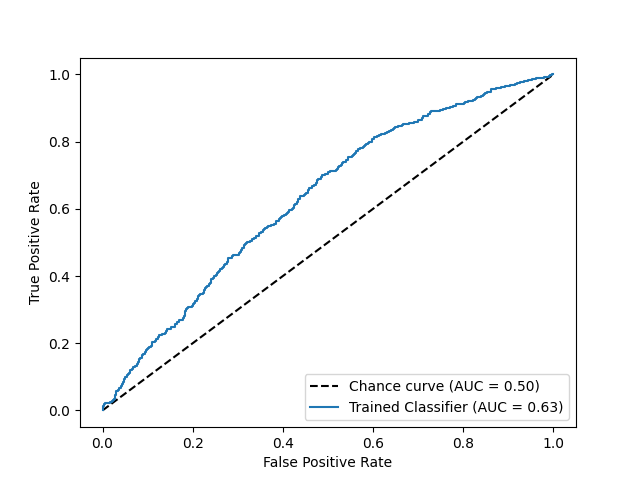
\includegraphics[width=0.3\textwidth]{Figures/07/sample_auc/biolinkbert_pet_50_trafilatura_title_dev_ROC_on_split.png}
    }
    \hfill
    \subfigure[\bertroberta{} with \petTwoHundred{} on the \trafilaturaFulltext{}]{
            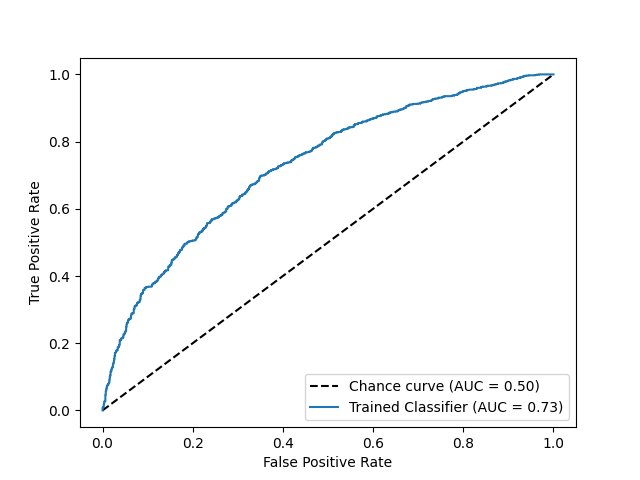
\includegraphics[width=0.3\textwidth]{Figures/07/sample_auc/roberta_pet_200_trafilatura_fulltext_dev_ROC_on_split.png}
    }
    \hfill
    \subfigure[\bertxlmroberta{} with \petThousand{} on the \trafilaturaFulltext{} ]{
            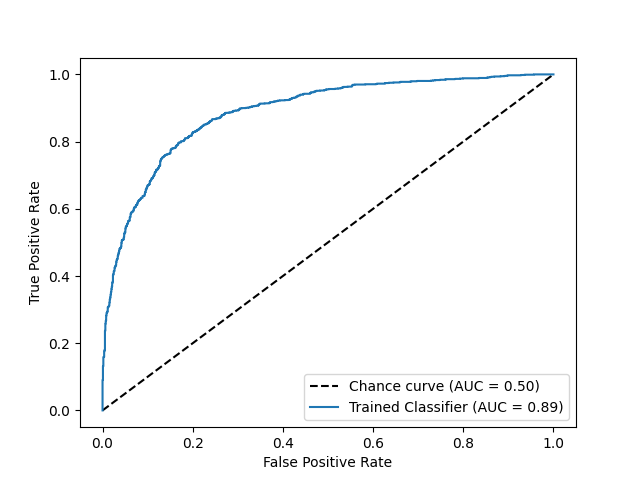
\includegraphics[width=0.3\textwidth]{Figures/07/sample_auc/xlmroberta_pet_1000_fulltext_dev_ROC_on_split.png}
    }
    \caption{Sample \auc{}s for some classifiers}
    \label{fig:07_vsi_sample_auc}
\end{figure}


Prioritizing models that genuinely grasp the concept of relevance rather than indiscriminately marking everything as positive, we set a threshold of 80\% for the Development \auc{}. By doing so, we narrow down to 49 classifiers, detailed in Table \ref{appendix05:tab:f2_auc_f1_top_pergorming_by_content_type}.
Interestingly, the \contentType{} with the highest number of top-performing classifiers is the \trafilaturaFulltext{}, exhibiting 15 top classifiers across all \gls{bert} models.
This indicates that the \trafilaturaFulltext{}, typically longer than other \contentType{}s, offers ample content, enabling all models to effectively learn the task.

Conversely, it's worth noting that the \keyphrasesAbstractOnly{} doesn't feature on the list. 
As discussed in \headerName{} \ref{vsi_preprocessing}, this dataset undergoes significant reduction during preprocessing, potentially leaving it with insufficient content.
Given that we still have four top-performing classifiers for the \trafilaturaAbstract{}, we opt to \textbf{exclude} the \keyphrasesAbstractOnly{} as a \contentType{}.


To avoid classifiers that flag almost everything as a positive, we impose a 75\% threshold on the Development \fOne{}.
This criterion narrows our selection to 17 classifiers. 
Table \ref{appendix05:tab:metrics_for_best_classifiers} presents the Development and Test metrics for these classifiers, emphasizing the top-performing metrics.
Once more, the \trafilaturaFulltext{} dominates with the most classifiers on this list (9), and its best three metrics are highlighted.

Predictably, the Test metrics are lower than the Development metrics. 
Yet, it's striking to see a significant drop in the \fOne{} and precision, with most falling below the 50\% mark. 
This trend can be attributed to our emphasis on the \fTwo{}, which leans towards Recall at the expense of Precision. At the same time, the highest Test Recalls hover around or exceed 80\%.


Observe that the \keyphrasesFulltextOnly{} is absent from the list. 
This can be attributed to the significant reduction in dataset content when only sentences containing keywords are considered. 
Additionally, the peak metrics for \keyphrasesAbstractOC{} and \keyphrasesFulltextOC{} consistently fall short of those for \trafilaturaAbstract{} and \trafilaturaFulltext{}, respectively.
These findings suggest that incorporating \keyphrases{} as \contentType{}s does \textbf{not} enhance performance, contrary to our hypothesis in \headerName{} \ref{vsi_leveraging_keywords}. 
Consequently, we opt to \textbf{exclude} these sources of content moving forward, and thus, we are left with the four original \contentType{}s.


Considering the best performing classifiers (Table \ref{tab:07_best_classifiers}), it's noteworthy that, except for one, all top classifiers are derived from \petThousand{}.
Moreover, the best classifiers are consistently obtained by training multilingual \gls{bert} models. This highlights the significance of the multilingual nature of our dataset in determining relevance over its biomedical aspect.


\begin{table}[ht]
\resizebox{\textwidth}{!}{
\begin{tabular}{|l|c|c|ccc|c|}
\hline
\contentType{}       & \trafilaturaTitle{}    & \trafilaturaAbstract{}    & \trafilaturaFulltext{} & \trafilaturaFulltext{}           & \trafilaturaFulltext{}   & \translationTitle{} \\ 
Model           & \bertmultilingual{}                 & \bertxlmroberta{}           & \bertmultilingual{}                 & \bertxlmroberta{}           & \bertxlmroberta{}           & \bertmultilingual{}                 \\
Training Method & \petThousand{}              & \petThousand{}              & \petThousand{}              & \balanced{}   & \petThousand{}              & \petThousand{}              \\ \hline
Development \fTwo{}  & \mycoloredcell{0.8244310265} & \mycoloredcell{0.8233701782} & \mycoloredcell{0.8274771609} & \mycoloredcell{0.8361531612} & \mycoloredcell{0.8573388203} & \mycoloredcell{0.8286908078} \\
Development \auc{}       & \mycoloredcell{0.8345520661} & \mycoloredcell{0.8415276893} & \mycoloredcell{0.8882393048} & \mycoloredcell{0.9057368386} & \mycoloredcell{0.8884577866} & \mycoloredcell{0.8526575213} \\
Development \fOne{}  & \mycoloredcell{0.7755324959} & \mycoloredcell{0.7741251326} & \mycoloredcell{0.8152315015} & \mycoloredcell{0.8395172105} & \mycoloredcell{0.8159934721} & \mycoloredcell{0.7880794702} \\
Development Accuracy  & \mycoloredcell{0.7509090909} & \mycoloredcell{0.7491166078} & \mycoloredcell{0.8105590062} & \mycoloredcell{0.8405861456} & \mycoloredcell{0.7999112689} & \mycoloredcell{0.7692307692} \\
Development Precision & \mycoloredcell{0.7057654076} & \mycoloredcell{0.7039537126} & \mycoloredcell{0.7956081081} & \mycoloredcell{0.8451845185} & \mycoloredcell{0.7552870091} & \mycoloredcell{0.7285714286} \\
Development Recall    & \mycoloredcell{0.8606060606} & \mycoloredcell{0.8598351001} & \mycoloredcell{0.8358473824} & \mycoloredcell{0.8339253996} & \mycoloredcell{0.8873114463} & \mycoloredcell{0.8581730769} \\ \hline
Test \fTwo{}         & \mycoloredcell{0.6055995131} & \mycoloredcell{0.6056860321} & \mycoloredcell{0.6696935301} & \mycoloredcell{0.637195122}  & \mycoloredcell{0.6379132231} & \mycoloredcell{0.6380890052} \\
Test \auc{}        & \mycoloredcell{0.8249796338} & \mycoloredcell{0.8460210289} & \mycoloredcell{0.8961402345} & \mycoloredcell{0.8721908143} & \mycoloredcell{0.896623166}  & \mycoloredcell{0.8419944312} \\
Test Precision  & \mycoloredcell{0.2783216783} & \mycoloredcell{0.2873900293} & \mycoloredcell{0.5021276596} & \mycoloredcell{0.511002445}  & \mycoloredcell{0.4434470377} & \mycoloredcell{0.318627451}  \\
Test Recall     & \mycoloredcell{0.8577586207} & \mycoloredcell{0.8376068376} & \mycoloredcell{0.7923691216} & \mycoloredcell{0.8223801066} & \mycoloredcell{0.7249334516} & \mycoloredcell{0.8515283843} \\
Test \fOne{}         & \mycoloredcell{0.4202745512} & \mycoloredcell{0.4279475983} & \mycoloredcell{0.3543543544} & \mycoloredcell{0.3841911765} & \mycoloredcell{0.294047619}  & \mycoloredcell{0.4637336504} \\
Test Accuracy   & \mycoloredcell{0.6672727273} & \mycoloredcell{0.691401649}  & \mycoloredcell{0.8613138686} & \mycoloredcell{0.7627737226} & \mycoloredcell{0.901459854}  & \mycoloredcell{0.7289663462} \\ \hline
\end{tabular}
}
\caption{Best classifiers by \contentType{}}
\label{tab:07_best_classifiers}
\end{table}


\putInBox{

In summary, among all the training methods examined in our work, \unbalanced{} yields the least favorable performance, while \gls{pet} demonstrates increasingly improved performance as more documents per category are introduced. In terms of \contentType{}s, incorporating keywords from the documents does not enhance performance, whereas utilizing the \trafilaturaFulltext{} proves to be the most effective in providing substantial content for the models to learn from, with the \trafilaturaTitle{}, \translationTitle{} and \trafilaturaAbstract{} lagging behind. Additionally, the multilingual aspect of our dataset appears to hold greater significance than their biomedical content, as evidenced by the superior performance of classifiers trained with multilingual \gls{bert} models.


}


Finally, we put forward a reason for the enhanced performance of \gls{pet} compared to \finetuning{}. We theorize that the use of task descriptions in \gls{pet} enables the model to have a clearer comprehension of the task. To illustrate this idea, we reference an example from the foundational \gls{pet} paper by \mytextcite{pet_paper}.

Take into account the next three statements: the first two have labels, and our challenge is to assign a label to the third.


\begin{itemize}
    \item[1.] Category A: This \textit{was} the best \textit{pizza} I've ever had.
    \item[2.] Category B: You \textit{can} get better sushi for half the \textit{price}.
    \item[3.] Category ?: \textit{Pizza} \textit{was} average. Not worth the \textit{price}.
\end{itemize}
\vspace{4pt}

Based solely on this data, determining a label is challenging: Is the focus on pizza or price? Or is it about identifying verb tenses (Past vs. Present)? Yet, if we're informed that the objective is to identify sentences discussing pizza, we'd promptly label the third sentence in category A. Conversely, if it's about prices, category B would be the appropriate label. 

For our task, consider the three following (artificial) sentences:
\begin{itemize}
    \item[1.] Relevant: Oriental Fruit fly (Bactrocera dorsalis) detected in a new location in Central Asia.
    \item[2.] Irrelevant: Check out the best decorative plants for your garden this summer, and beware of insects! 
    \item[3.] Category ?: What to do if you find fruit flies plaguing your field - Agriculture News Online. 
\end{itemize}
\vspace{4pt}

For the task of identifying document relevance for Plant Health Surveillance, we categorize the third sentence as 'Irrelevant'. However, such subtleties might be overlooked by a language model without additional context.


Indeed, referring to Table \ref{tab:07_best_classifiers}, it's evident that \finetuning{} yields one of the top classifiers only when applied to the \trafilaturaFulltext{}. 
Throughout our analysis, we've observed that many top-performing classifiers were also trained on the \trafilaturaFulltext{}. 
This suggests that due to its length (averaging 1102 tokens, but cut at 300 input tokens), the \trafilaturaFulltext{} provides ample content, enabling any \gls{bert} model to grasp the task effectively.
In contrast, other \contentType{}s, being much shorter than the \trafilaturaFulltext{}, might not offer sufficient context for the models. For instance, the \trafilaturaTitle{} averages 11 tokens, the \trafilaturaAbstract{} 50 tokens, and the \translationTitle{} 12 tokens. 
As a result, classifiers benefit from the added context given by \gls{pet} patterns.

Furthermore, it's worth noting that all other best classifiers predominantly use \petThousand{}. 
This suggests that exposing the model to more document examples combined with task-specific knowledge enhances its performance.
However, the performance improvement stales over time, as the incremental gains from transitioning from \petFiveHundred{} to \petThousand{} are marginal, as seen in Tables \ref{tab:07_f2_bert_base}-\ref{tab:07_f2_bert_xlmroberta}.

In conclusion, by employing \gls{pet} and its patterns, we inject task-specific knowledge, thereby guiding the model. 


\clearpage